\section{Results}

All the following benchmarks were conducted on a Github-hosted virtual machine
under GitHub Actions, running Ubuntu 22.04 LTS with a 4-core, 8-thread CPU and
16GB of RAM\@. All tests were conducted on the OpenJDK VM Corretto 21. The JVM
was configured with a minimum heap size of 512MB and a maximum heap size of
16GB\@.

For both the Apache Bench and JMeter tests, we simulate a 1000-request warmup
period for each route with a concurrent user load of 32 users. The warmup
period is followed by the actual test period, during which we simulate 256
requests per user, scaling in increments up to 128 concurrent users.

The results are presented in the form of throughput (number of requests per
second) for each template engine, with the x-axis representing the number of
concurrent users and the y-axis representing the throughput in requests per
second.

Both the Quarkus and Spring MVC implementations were configured with an output
buffer size of 8KB, despite the Quarkus implementation not enabling PSSR at
this size. This configuration was chosen to ensure consistency across Spring
MVC and Quarkus, as the Spring MVC implementation does not support PSSR for the
tested templates.

Since the obtained results for JMeter and Apache Bench show no significant
differences, only the JMeter results will be presented.

\subsection{Presentations Results}

The results in Figure~\ref{fig:presentations-webflux-jmeter} depict the
throughput (number of requests per second) for each template engine, with
concurrent users ranging from 1 to 128, from left to right. The benchmarks
include HtmlFlow using suspendable web templates (\textit{HtmlFlow-Susp},
equivalent to the approach shown in Listing~\ref{lst:presentation-flow}),
Jstachio using Virtual Threads with the \texttt{Iterable} interface
(\textit{Jstachio-Virtual}), and Thymeleaf using the reactive View Resolver
driver (Thymeleaf-Rx). \textit{Blocking} and \textit{Virtual} represent the
average throughput of the blocking approaches (i.e., KotlinX, Rocker, Jstachio,
Pebble, Freemarker, Trimou, HtmlFlow, and Thymeleaf) when run in the context of
a separate coroutine dispatcher or Virtual Threads, respectively.

We show the \textit{HtmlFlow-Susp}, \textit{Jstachio-Virtual}, and
\textit{Thymeleaf-Rx} engines separately to observe the performance of the
non-blocking engines when using the Suspending, Virtual Thread, and Reactive
approaches. The \textit{Blocking} and \textit{Virtual} are aggregated due to
the similar performance of different engines when using those approaches.

\begin{figure}[h]
     \centering
     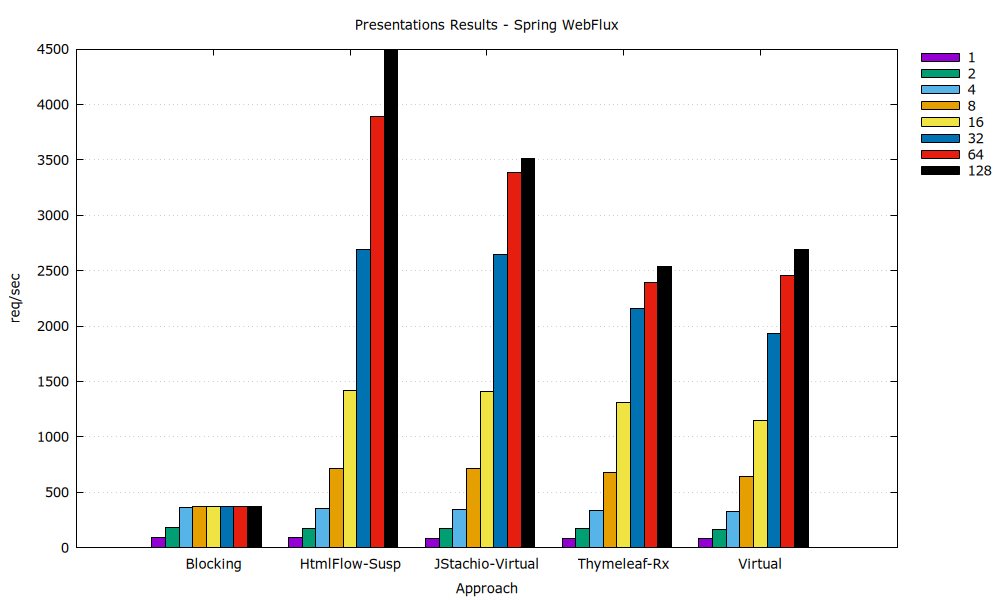
\includegraphics[width=0.8\textwidth]{./Graphs/presentations-webflux-jmeter.png}
     \caption{Presentation Benchmark Results in Spring WebFlux with JMeter}\label{fig:presentations-webflux-jmeter}
\end{figure}

The results in Figure~\ref{fig:presentations-webflux-jmeter} show that when
using blocking template engines with a separate coroutine dispatcher, the
engines are unable to scale effectively beyond 4 concurrent users. In contrast,
the non-blocking engines scale efficiently up to 128 concurrent users, with
HtmlFlow achieving 4,487 requests per second. When blocking approaches are
executed in the context of Virtual Threads—thus enabling non-blocking I/O—the
engines also scale up to 128 concurrent users, with Jstachio using Virtual
Threads reaching 3,514 requests per second. The Thymeleaf implementation using
the reactive View Resolver driver also scales up to 128 concurrent users, but
achieves a lower throughput of approximately 2,559 requests per second.

It is important to note that the differences in scalability and throughput
between the \textit{HtmlFlow-Susp}, \textit{Jstachio-Virtual}, and
\textit{Thymeleaf-Rx} approaches may be influenced by the specific template
engines used, rather than the approach itself. When comparing the
\textit{Reactive}, \textit{Suspendable}, and \textit{Virtual} approaches
specifically with HtmlFlow, we found that all three achieve similar
performance: HtmlFlow using a blocking approach with Virtual Threads reaches
4,691 requests per second, while HtmlFlow using a reactive approach achieves
4,792 requests per second.

\begin{figure}[h]
     \centering
     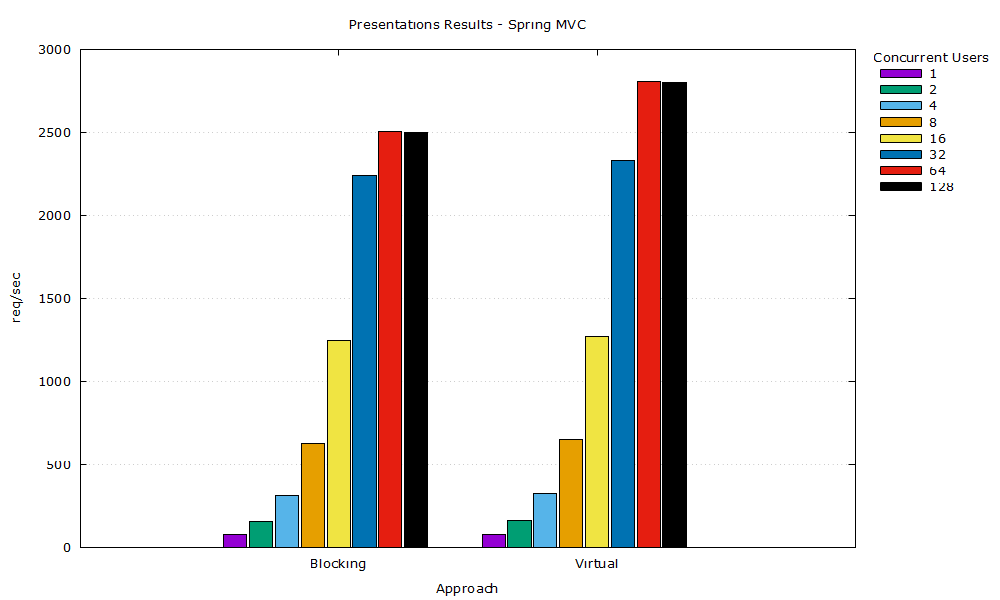
\includegraphics[width=0.8\textwidth]{./Graphs/presentations-springmvc-jmeter.png}
     \caption{Presentation Benchmark Results in Spring MVC with JMeter}\label{fig:presentations-springmvc-jmeter}
\end{figure}

% The results for the Spring MVC implementation, shown in
% Figure~\ref{fig:presentations-springmvc-jmeter}, compare two approaches:
% \textit{Blocking}, which uses platform threads with \texttt{StreamingResponseBody},
% and \textit{Virtual}, which uses Virtual Threads. Both approaches scale
% effectively up to 128 concurrent users, with the Virtual Thread approach
% achieving a slightly higher throughput of 9,000 requests per second. However,
% these values are slightly lower than those observed in the Spring WebFlux
% implementation.
The results for the Spring MVC implementation, shown in
Figure~\ref{fig:presentations-springmvc-jmeter}, compare two synchronous
approaches: \textit{Blocking}, which uses platform threads with
\texttt{StreamingResponseBody}, and \textit{Virtual}, which uses Virtual
Threads. Since Spring MVC follows a thread-per-request architecture, the
asynchronous approaches—\textbf{Reactive} and \textbf{Suspendable}—described in
Section~\ref{sec:bench} are not applicable. Both the \textit{Blocking} and
\textit{Virtual} strategies scale effectively up to 128 concurrent users, with
the Virtual Threads approach achieving a slightly higher maximum throughput of
2,797 requests per second, compared to 2,498 requests per second for the
blocking approach. These results indicate that while Spring MVC can handle a
moderate level of concurrency, it does not reach the scalability of the
reactive or suspendable approaches available in Spring WebFlux. Furthermore,
Spring MVC does not enable Progressive Server-Side Rendering (PSSR) for the
tested templates, as previously discussed in Section~\ref{sec:bench}.

\begin{figure}[h]
     \centering
     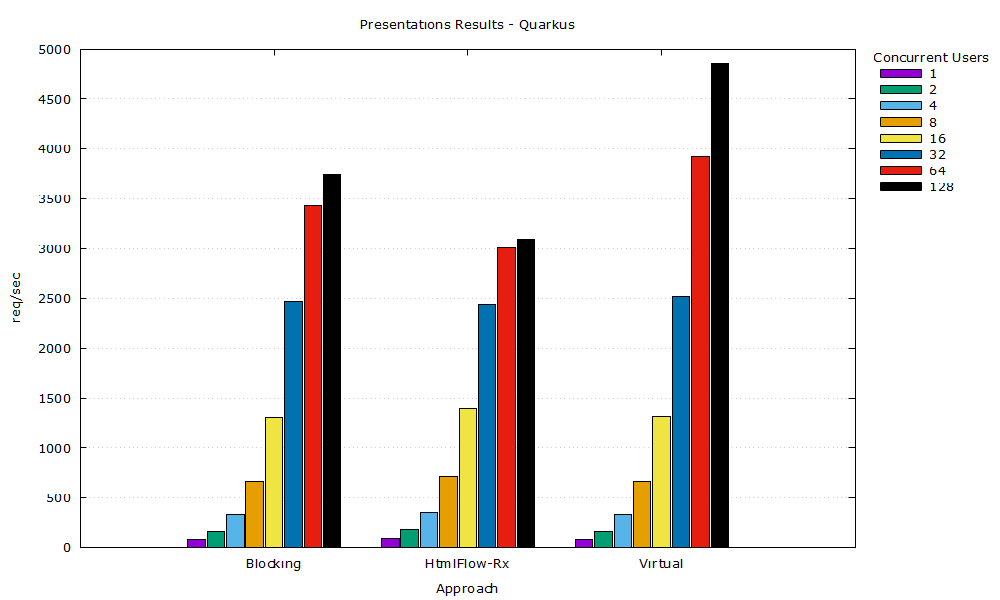
\includegraphics[width=0.8\textwidth]{./Graphs/presentations-quarkus-jmeter.png}
     \caption{Presentation Benchmark Results in Quarkus with JMeter}\label{fig:presentations-quarkus-jmeter}
\end{figure}

The results for the Quarkus implementation, shown in
Figure~\ref{fig:presentations-quarkus-jmeter}, indicate that Quarkus handles
synchronous approaches more efficiently than Spring WebFlux. The blocking
engines scale up to 128 concurrent users, achieving up to 3744 requests per
second. When using Virtual Threads, the throughput increases even further,
reaching 4856 requests per second. This demonstrates that Quarkus's
implementation of Virtual Threads is effective for enabling PSSR\@, and
comparable to the \textit{Suspendable} and \textit{Reactive} used approaches in
Spring WebFlux in terms of scalability and throughput.

Additionally, \textit{HtmlFlow-Rx}, a reactive implementation of the HtmlFlow
template engine (equivalent to the approach shown in
Listing~\ref{lst:presentation-observable}) that utilizes Quarkus's reactive
programming model, achieved a lower throughput than the the \textit{Blocking}
and \textit{Virtual} approaches—3088 requests per second. This demonstrates
that Quarkus's reactive programming model is effective for enabling PSSR\@,
although it does not achieve the same level of performance as the same approach
in Spring WebFlux.

\subsection{Stocks Results}

\begin{figure}[h]
     \centering
     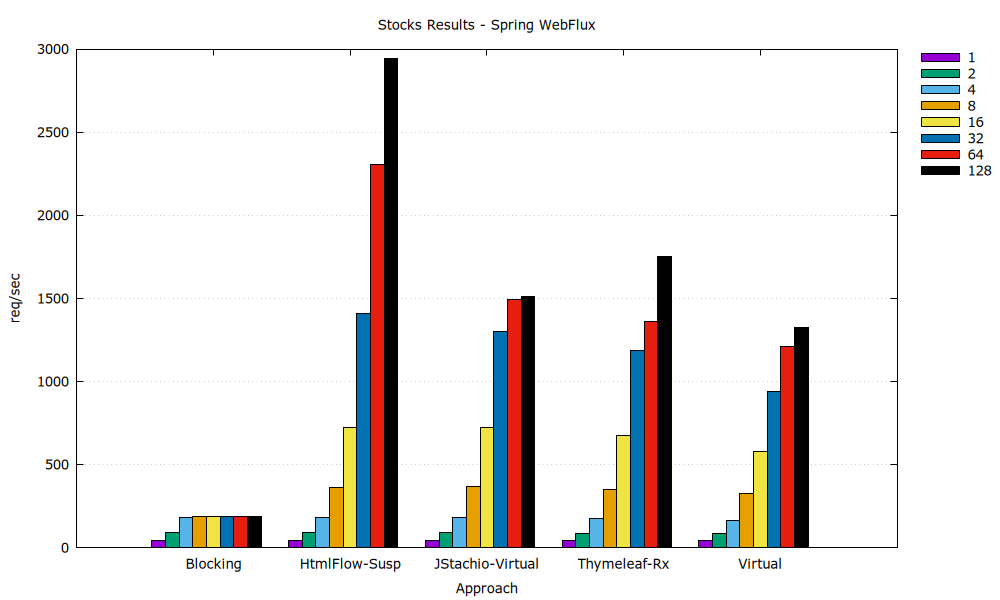
\includegraphics[width=0.8\textwidth]{./Graphs/stocks-webflux-jmeter.png}
     \caption{Stocks Benchmark Results in Spring WebFlux with JMeter}\label{fig:stocks-webflux-jmeter}
\end{figure}

The results in Figure~\ref{fig:stocks-webflux-jmeter} use the same template
engines and approaches as the previous benchmark, but replace the data model
with the more complex Stock class, including 20 instances. When using this data
model, we observe that the scalability of the engines is not significantly
affected, however the throughput is reduced across all engines. When compared
to the Presentation benchmark, we observe that particularly the approaches
using Virtual Threads took a greater performance hit when compared to the
\textit{Reactive} and \textit{Suspending} approaches, with Jstachio using
Virtual Threads now achieving 1509 requests per second, compared to the 1,750
requests per achieved by the Thymeleaf implementation using the reactive View
Resolver driver.

It is again important to note that the differences in scalability and
throughput between the \textit{HtmlFlow-Susp}, \textit{Jstachio-Virtual}, and
\textit{Thymeleaf-Rx} approaches may be influenced by the specific template
engines used, rather than the approach itself. When comparing the
\textit{Reactive}, \textit{Suspendable}, and \textit{Virtual} approaches
specifically with HtmlFlow, we found that all three achieve similar
performance: HtmlFlow using a blocking approach with Virtual Threads reaches
3,090 requests per second, while HtmlFlow using a reactive approach achieves
3,026 requests per second.

The overall throughput reduction is expected, as the Stock class contains more
data properties than the \texttt{Presentation} class, adding overhead related
to the data binding process of each template engine.

\begin{figure}[h]
     \centering
     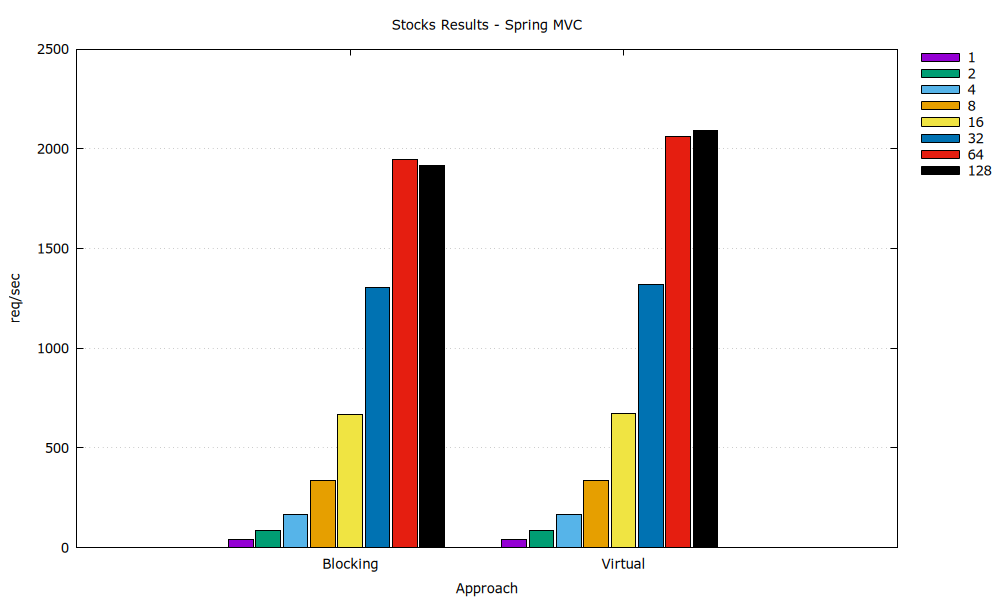
\includegraphics[width=0.8\textwidth]{./Graphs/stocks-springmvc-jmeter.png}
     \caption{Stocks Benchmark Results in Spring MVC with JMeter}\label{fig:stocks-springmvc-jmeter}
\end{figure}

The results shown in Figure~\ref{fig:stocks-springmvc-jmeter} indicate that the
Spring MVC implementation using the blocking approach with
\texttt{StreamingResponseBody} achieves a throughput of up to 1,916 requests
per second, with no significant improvement observed when using Virtual
Threads. Both approaches scale effectively up to 128 concurrent users. Although
these approaches achieve higher throughput in Spring MVC than in Spring
WebFlux, their overall performance remains lower than that of the reactive and
suspendable approaches.

\begin{figure}[h]
     \centering
     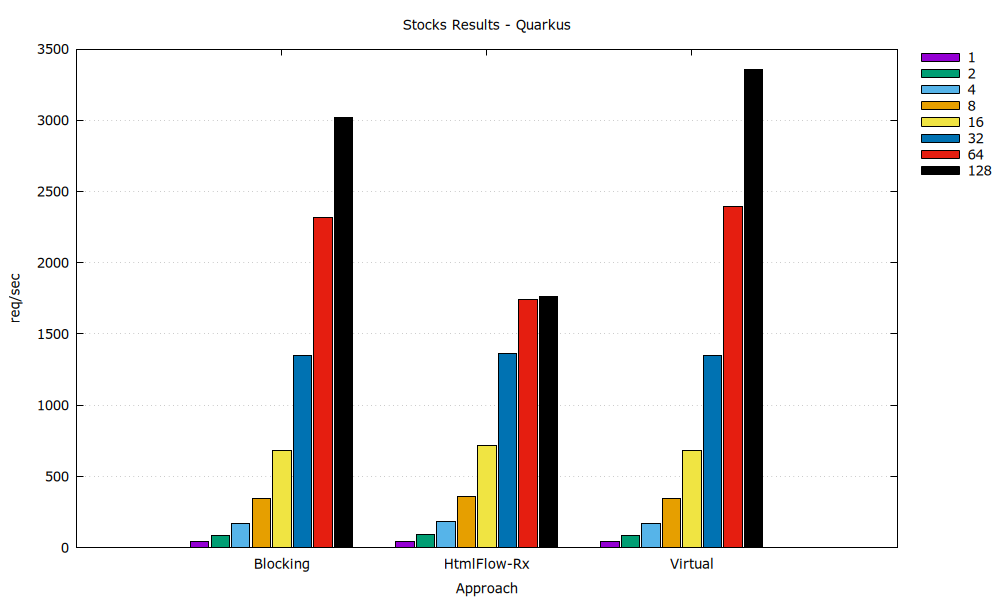
\includegraphics[width=0.8\textwidth]{./Graphs/stocks-quarkus-jmeter.png}
     \caption{Stocks Benchmark Results in Quarkus with JMeter}\label{fig:stocks-quarkus-jmeter}
\end{figure}

The results depicted in Figure~\ref{fig:stocks-quarkus-jmeter} show that the
Quarkus implementation scales effectively up to 128 concurrent users, achieving
performance comparable to the Spring WebFlux implementation. The blocking
approach reaches a throughput of 3,019 requests per second, while the Virtual
Threads approach achieves a throughput of 3,357 requests per second.

In addition to the blocking engines, the \textit{HtmlFlow-Rx} approach also
achieves a throughput of 1760 requests per second, indicating that this
approach achieves lower performance in Quarkus than in Spring WebFlux, where it
reached 3,026 requests per second, as previously mentioned.

The results of the benchmarks show that non-blocking engines, through the use
of reactive programming, Kotlin coroutines, or Java virtual threads, are able
to scale effectively up to 128 concurrent users. Out of all the tested
frameworks, Spring Webflux showed itself the most effective at enabling PSSR,
mostly due to its native support for Publish and Subscriber interfaces, which
allow for HTML content to be progressively streamed to the client. Quarkus also
enabled PSSR effectively, but it required additional configuration of the
\texttt{OutputBuffer} size to achieve the same results as Spring Webflux. The
Spring MVC implementation, on the other hand, did not enable PSSR for the
tested templates.

Additionally, the results show that approaches using Virtual Threads are able
to scale as effectively as those using reactive programming or Kotlin
coroutines, allowing \textit{external} DSLs to be used in a non-blocking
context, effectively enabling PSSR\@.